\section{Experimental evaluation}
%\label{sec:context}

\subsection{Dataset composition}
The dataset taken into account during the experimental evaluation is composed both by \textbf{real} and \textbf{synthetic} data organized in ".csv" files. In particular the \textbf{Relational Table} $RT$ is composed by real data that, in the scenario considered, represents 7669 existing movies. The movies taken into account were retrieved from kaggle.com, a popular collection of public datasets used for data science works. The dataset was moreover cleaned and projected in the tuple $\langle name, genre, runtime, year, country, score \rangle$ \\in order to make it compatible with the other synthetic data used.
The \textbf{User Set} $US$, the \textbf{Query Set} $QS$ and the \textbf{Utility Matrix} $U$ are instead synthetic and were generated by the team. In particular:
\begin{itemize}
    \item The \textbf{User Set} is composed by a list of 2500 users' ids generated through the use of the $uuid$ python's module. Each user has an \textbf{unspoken preference} regarding each attribute belonging to the items' tuple in order to generate the utility matrix in a \textbf{coherent} way. 
    \item The \textbf{Query Set} is composed by 100 queries. Each query is represented by at least a key-value constraints, where each one of them corresponds to existing attribute and value present in at least a tuple of the Relational Table $RT$. 
    \item The \textbf{Utility Matrix} is composed by a matrix having $u$ rows, with $u$ corresponding to the number of users, and $q$ columns, with $q$ corresponding to the number of queries. \textbf{One third} of the user-query combinations of the matrix is filled with a rating computed by taking into account the unspoken user preferences on the results produced by the execution of the queries on the relational table.
\end{itemize}
The \textit{Complete Utility Matrix}, composed by the Utility Matrix $U$ without any hidden value, was also stored in order to use it only during the \textbf{performance evaluation} of the proposed solution and of the ones produced by the baselines considered.

\subsection{Dataset generation} \label{ch:5.2}
The synthetic data of the dataset considered were generated in order to accomplish the attributes and values of the real relational table. Another choice taken, in order to work on a dataset having as \textbf{few assumptions} as possible and so whose solution would work in the same way also with other ones, was to do \textbf{not} establish any correlation through different distances between the values belonging to discrete fields. For instance, in the current scenario, the Thriller genre could have been considered a closer concept to the Horror genre than the Musical genre.

\subsubsection{Fields recognition}
In order to generate the data in this way, first of all it was necessary to analyze the kind of attributes belonging to the real relational table and to divide them in:
\begin{itemize}
    \item \textbf{Discrete Attribute} (as the genre and the country)
    \item \textbf{Continuous Attributes} (as the runtime, the publication year and the score)
    \item \textbf{Not-relevant attributes} (as the "name")
\end{itemize}
In order to do that, the distinction was computed by considering at first the attributes where each of their value could be parsed in a numeric format. Those fields were considered as \textbf{continuous}. The non-continuous fields, in addition, were divided in \textbf{not-relevant} attributes, in the case they were unique in at least the 75\% of the times, and \textbf{discrete}, otherwise. During the generation of the dataset it is also given the possibility of specifying manually which continuous fields will influence the user ratings in the same way for everyone, for example in the current relational table the field "score" (like a IMDB score) will influence everyone \textbf{in the same way} by increasing or decreasing the rating given to an item independently by the users' preferences.

\subsubsection{User profiles}
Once the fields were divided in this way, they were leveraged in order to build the users' profiles. Each user's profile is characterized by:
\begin{itemize}
    \item a \textbf{user\_id}, which represents the only known field about the user used by the actual solution algorithm.
    \item an \textbf{average\_score\_translation} field, a random value between -10 and 10 that will indicate if a user is \textbf{severe or not} in his rating.
    \item \textbf{10 fields for every discrete field} of the relational table, in order to indicate which are the values for those fields that a user will \textbf{appreciate} the most (the first 4 ones) or the least (the last 6 ones). The values not present in the user profile will be simply rated as unpleasant, with a contribution of 60 out of 100 each.
    \item \textbf{a field for every continuous attribute} regarding the items (except for the score one), in order to express the users' unspoken preferences toward a certain continuous item field. Those preferences contains a value picked from a \textbf{Gaussian distribution} having as mean the mean value regarding a certain continuous attribute and with a standard deviation such that over the 98,5\% of the values will be in the range of values found in the relational table for each attribute. It was chosen to use a Gaussian distribution in order to generate those preferences by also managing the existence of very high or very low values appearing in the big minority of the items considered. If it was chosen to pick some random equiprobable values for computing the users' preferences between the real range of values, a big amount of those picks will be strongly similar to only few (usually one) items of the relational table.
\end{itemize}
Those users profiles built were used both in the creation of the Utility Matrix $U$ belonging to the input of the problem, both during the evaluation performed for the PART\_B of the solution proposed.

\subsubsection{Query definition}
It was then built the definition of the attribute-value constraints belonging to 100 queries that will compose the columns of the utility matrix proposed. In order to reduce the number of queries that won't return any result if executed on the Relational Table $RT$, after having picked a attribute-value constraint referring to a considered field present in the relational table, the other ones were added with 25\% of probability each. The combination of those constraints will represent our query definition.

\subsubsection{Query result computation}
As a pre-computation used during the creation of the Utility Matrix, each query was computed on the entire relational table and its results were saved in a file called \textit{*query\_id*.csv}. This operation was simply done by iterating over all the attribute-value pairs defined for each query and by writing to file the items that were satisfying all of it.

\subsubsection{Utility matrix computation}
With all those computations performed, it is actually possible to compute both the \textit{Real Utility Matrix}, a complete matrix containing the ratings of all the users for all the queries, both the \textit{Utility Matrix} $U$, that represents an \textbf{input} of our problem statement.
In order to compute them, an iteration through all the users and all the query results achieved was performed and it was assigned, using the unspoken preferences of the users, a rating for each query. The rating of a query by a user corresponded to the \textbf{mean} of all the ratings that the user gave to its \textbf{results}. The rating given to a single item by a user is obtained by the sum of:
\begin{itemize}
    \item the ratings given to each \textbf{discrete attribute} of the item. Those ratings depend by the position of which the effective discrete value of an item appears in the user profile.
    \item the ratings given to each \textbf{continuous attribute} of the item. Those ratings depend on the distance between the value characterizing an item and the one presents in the user preferences. It was chosen to use an arithmetic distance normalized considering the values' spectrum of each attribute taken into account in order to obtain a preference score between 0 and 100. This distance obtained it was furthermore subtracted to 100 in order to have an higher value when the user profile and the item's one were similar.
    \item a value indicating how the item in account was \textbf{generally} appreciated. This value is represented, in our case, by the $score$ field that can also influence negatively the rating assigned to an item. This field was normalized in order to give to it the possibility to add a value between -7,5 and 7,5 to the final score assigned to the item.
\end{itemize}
After having summed up the previous values, the final result was normalized in order to obtain a value between \textbf{0 and 100} by dividing it by the number of the considered items' fields taken into account (excluded the \textit{score} one that was managed in a different way). The case in which a rating was still over 100 or under 0 were shifted respectively to 100 and to 0.

The mean of the ratings, belonging to items composing the results of the same query, will \textbf{compose the rating} assigned by a user to the query taken into account. In order to provide more variety between the queries ratings assigned by different users, it was furthermore added to it:
\begin{itemize}
    \item the \textit{average\_score\_translation} belonging to each user profile, a value between -10 and 10 used to indicate if a user is \textbf{severe or not} in his reviews.
    \item a \textbf{random noise} between -5 and 5, in order to get less predictable results.
\end{itemize}
Also this obtained rating was shifted in order to get a value between 0 and 100. The pseudocode related to this rating-computation procedure is illustrated with Algorithm \ref{alg:users-queries score computation}.

\begin{algorithm}
\caption{Utility Matrix and Complete Utility Matrix Computation}
\label{alg:users-queries score computation}
\KwData{users,query\_results (by reading each \textit{*query\_id*.csv}),queries,utility\_matrix,preprocessed\_queries, DISC\_FIELDS,CONT\_FIELDS,SCORE}
\KwResult{utility\_matrix,complete\_utility\_matrix}

complete\_utility\_matrix[][] \\
utility\_matrix[][] \\

\For{user \textbf{in} users}{ 
    \For{query \textbf{in} queries}{ 
        partial\_query\_rating=0 \\
        \For{item \textbf{in} query\_results[query]}{
            partial\_item\_rating=0 
            
            \For{field \textbf{in} item}{ 
                \If{field in DISC\_FIELDS}{ 
                    partial\_query\_rating+= compute\_discrete(user[field],item[field]) 
                }
                \uIf{field in CONT\_FIELDS \&\& field \textbf{not in} SCORE}{ 
                    partial\_query\_rating+= compute\_continuous(user[field],item[field]) 
                }\Else{ 
                    partial\_query\_rating+= compute\_score(item[field]) 
                }
            } 
        } 

        partial\_query\_rating+= partial\_item\_rating / (|DISCR\_FIELD|+| CONT\_FIELDS|-|SCORE|)

    partial\_query\_rating=partial\_query\_rating / query\_results[query].len() 
    
    partial\_query\_rating+=user["average\_score\_translation"] 
    
    final\_query\_rating=partial\_query\_rating+random(-5,5) 
    
    complete\_utility\_matrix[user][query] = final\_query\_rating
    
    \If{random(1,3)==1}{ 
        utility\_matrix[user][query] = final\_query\_rating 
    } 
    }
        
} 

%return partial\_utility\_matrix,real\_complete\_utility\_matrix

\end{algorithm}





The \textit{compute\_discrete(user[field],item[field])} function in \ref{alg:users-queries score computation} checks in which position, if it exists, a discrete value of the relational tuple appears in the user profile. In particular, if a value appears in the first 4 positions of the user profile regarding the attribute considered, the rating given is between 100 and 70, according to its exact position. If the value instead appears in the last 6 positions, the rating given is poor, between 50 and 0. If the rating regarding a value does not appear in the user profile, it has a \textbf{standard contribution} of 60.
\textit{compute\_continuous(user[field],item[field])} is a function that computes the rating contribution regarding a continuous field that characterize the relational table in this way:
$$100-\frac{(abs(float(item[field])-float(user[field]))}{((max(field)-min(field))/100))}$$
So, it computes an arithmetic distance between the user preference and the item value regarding the same continuous field and it normalizes it in order to obtain a value between 0 and 100. It is also computed the complementary of this distance in order to obtain a similarity value.

\textit{compute\_score(item[field])} normalize the \textit{item[field]} in a value between -7.5 and 7.5. 

Finally, because the scores (belonging to the "score" field) in our dataset were between 0 and 5, the relative computation was performed in the following way:
$$(float(item[field])-2.5)*3$$

In this way, it is possible to compute all the ratings belonging to each user-query combination that will be part of the real and complete utility matrix used during the evaluation process. By \textbf{randomly keeping only the 33\%} of those ratings it is possible to obtain, instead, the Utility Matrix $U$ used during the solution's idealization.

\subsection{Dataset independence}

The solution provided is \textbf{independent} from the default input dataset.
This priority in building a general solution was considered since the \textbf{dataset generation}, whose algorithm adapts itself based on the type of values present in the \textbf{relational table} proposed as starting point. With the same approach, were also developed all the strategies that were tried for both the PART\_A and the PART\_B of the problem statement such that, every input given with the requested ".csv" representation, will be accepted independently by its fields and its cardinality.


\subsection{Evaluation metrics}
\label{sec:evaluation-metrics}

The evaluation metrics taken into account were:
\begin{itemize}
  \item \textbf{Mean Absolute Error} (MAE)
  \item \textbf{Root Mean Squared Error} (RMSE)
  \item \textbf{Mean Absolute Percentage Error} (MAPE)
\end{itemize}

\subsubsection{MAE}
In statistics, Mean Absolute Error (MAE) is a measure of errors between paired observations expressing the same phenomenon. \cite{MAE} In this particular case, Y versus X is the comparison of real value versus predicted. MAE is calculated as the sum of absolute errors divided by the sample size:

$$MAE = \frac{\sum ^{n}_{i=1} \left | y_{i} - x_{i} \right |}{n} = \frac{\sum ^{n}_{i=1} \left | e_{i}  \right |}{n}$$

In other words, its result show how close the predictions ($x_i$) are to the actual model ($y_i$) on average.
Low MAE values indicate that the model is correctly predicting. Larger MAE values indicate that the model is poor at prediction. \cite{metrics}

\subsubsection{RMSE}

The Root Mean Squared Error (RMSE) is the square root of the average of squared errors. The effect of each error on RMSE is proportional to the size of the squared error; thus RMSE is sensitive to \textbf{outliers}. \cite{RMSE}

$$RMSE = \sqrt{\frac{\sum_{t=1}^{N}(A_t - F_t)^{2}}{N}}$$

RMSE is used to determine whether there are any large errors or distances that could be caused if the model overestimated the prediction (that is, the model predicted values that were significantly higher than the actual values) or underestimated the predictions (that is, predicted values less than actual values). \cite{metrics}



\subsubsection{MAPE}

The Mean Absolute Percentage Error (MAPE) is another measure of prediction accuracy of a forecasting method in statistics. It usually expresses the accuracy as a ratio defined by the formula:

$$MAPE = \frac{100\%}{n} \sum_{t=1}^{n}\left | \frac{A_t - F_t}{A_t}  \right | $$

where $A_t$ is the actual value and $F_t$ is the forecast value. Their difference is divided by the actual value $A_t$. The absolute value of this ratio is summed for every forecasted point in time and divided by the number of points $n$.

According to some studies, a MAPE less than 5\% could be considered as an indication that the forecast is acceptably accurate. A MAPE greater than 10\% but less than 25\% could indicate low, but acceptable accuracy and MAPE greater than 25\% very low accuracy, so low that the forecast is not acceptable in terms of its accuracy. \cite{MAPE_VALUES}


These 3 metrics were used to \textbf{compare} the \textit{Real Complete Utility Matrix} (available right after the dataset generation) with the \textit{Complete Utility Matrix} computed by the final solution (Algorithm \ref{alg:hybrid}), and by the others approaches developed.

It should be noted that all of the aforementioned evaluation metrics are only ever used to compare two \textbf{full matrices}, one calculated by a developed component and the other created during the dataset generation phase.

In order to evaluate the tasks of PART\_A and PART\_B of the project, i.e., retrieve the \textit{TOP\_K} queries that may be of interest to the user $u$, \textbf{Jaccard similarity coefficient} were used.
This index is exploited to compare the \textbf{sets} of \textit{TOP\_K} queries computed from \textit{Real Complete Utility Matrix} and one computed with the developed algorithms.

\subsection{Experimental results accomplished by single components}

As said in the introduction of Chapter \ref{sec:solution}, the entire development process were driven not exclusively by reasoning deemed logical but also by empirical results. In this section, the \textbf{key experimental results} are reported.
Since the final solution relies on two separate components, it is helpful to examine their outcomes first.

\subsubsection{Compact Item-Item CF metrics values}

In order to determine the values of the three evaluation metrics mentioned in the previous section, the first experiments were carried out on the Compact Item-Item CF, the first component of the final solution.
Tables \ref{tab:compact Item-Item CF, nqueries fixed} and \ref{tab:compact Item-Item CF, nusers fixed} contain the results, and figures \ref{fig:Compact Item-Item CF, varying users} and \ref{fig:Compact Item-Item CF, varying queries} contain the relative plotted charts.
Regarding Figure \ref{fig:Compact Item-Item CF, varying users}, it is evident that all metrics considered in the chart reach a \textbf{plateau} after considering 200 users, even though the values are still slowly declining.
Figure \ref{fig:Compact Item-Item CF, varying queries} shows a slow decline in the metrics values rather than an initial steep section for the lower number of queries as there is for few users.

The data indicates that in order to reach a performance plateau, it is critical to cross a relatively consistent threshold of users, at least for this dataset. This behavior did not occur in the query variations considered.

\begin{table}[h!]
    \centering
    \begin{tabular}{ |p{2cm}||p{1.5cm}|p{1.5cm}|p{1.5cm}|  }
         \hline
         \multicolumn{4}{|c|}{Compact Item-Item CF, n\_queries (100) fixed } \\
         \hline
         \textbf{N\_USERS}& \textbf{MAE} &\textbf{RMSE} &\textbf{MAPE}\\
         \hline
         10 & 4.048 &  7.6871 & 8.7731\\
         20 & 3.7915 & 6.8982 & 8.2058\\
         50 & 3.6162 & 6.7762 & 8.3140\\
         100 & 3.3873 & 6.2586 & 7.5723\\
         200 & 3.3025 & 6.0730 & 7.2555\\
         300 & 3.2853 & 6.0379 & 7.2441\\
         400 & 3.2496 & 5.9567 & 7.1688\\
         500 & 3.2677 & 5.9896 & 7.2085\\
         1000 & 3.2384 & 5.9402 & 7.0622\\
         1500 & 3.2211 & 5.9151 & 7.0052\\ 
         2000 & 3.1691 & 5.8260 & 6.8783\\
         \textbf{2500} & \textbf{3.1420} & \textbf{5.7890} & \textbf{6.8218}\\
         
     
         \hline
    \end{tabular}
    \caption{Compact Item-Item CF, n\_queries fixed}
    \label{tab:compact Item-Item CF, nqueries fixed}
\end{table}


\begin{table}[h!]
    \centering
    \begin{tabular}{ |p{2cm}||p{1.5cm}|p{1.5cm}|p{1.5cm}|  }
         \hline
         \multicolumn{4}{|c|}{Compact Item-Item CF, n\_users (2500) fixed } \\
         \hline
         \textbf{N\_QUERIES}& \textbf{MAE} &\textbf{RMSE} &\textbf{MAPE}\\
         \hline
         10 & 3.2684 & 6.0499 & 7.5426\\
         20 & 3.1939 & 5.9215 & 7.3000\\
         30 & 3.1099 & 5.7911 & 7.0829\\
         40 & 3.0310 & 5.7740 & 7.2400\\
         50 & 3.2652 & 6.0235 & 7.2698\\
         60 & 3.3483 & 6.0666 & 7.1452\\
         70 & 3.1616 & 5.8735 & 7.0560\\
         80 & 3.2359 & 5.9161 & 6.9690\\
         90 & 3.2323 & 5.8874 & 6.8850\\
         \textbf{100}& \textbf{3.1420} & \textbf{5.7890} & \textbf{6.8218}\\
         
         \hline
    \end{tabular}
    \caption{Compact Item-Item CF, n\_users fixed}
    \label{tab:compact Item-Item CF, nusers fixed}
\end{table}

\begin{figure}[h!]
\centering
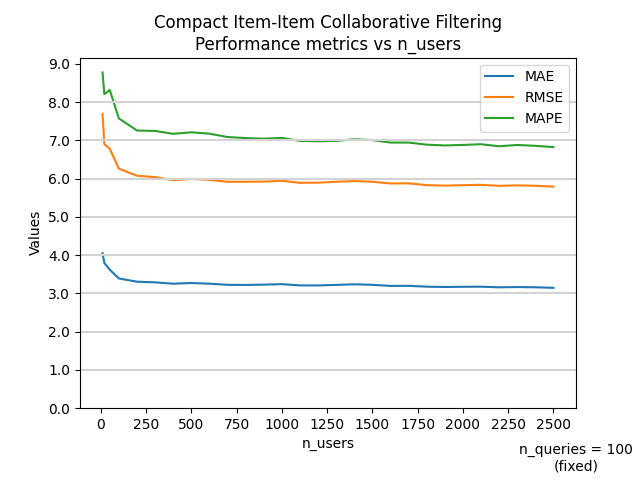
\includegraphics[width=9cm]{Data Mining/images/compact_item_item_users.png}
\caption{Evaluation metrics of Compact Item-Item CF, varying number of users}
\label{fig:Compact Item-Item CF, varying users}
\end{figure}

\begin{figure}[h!]
\centering
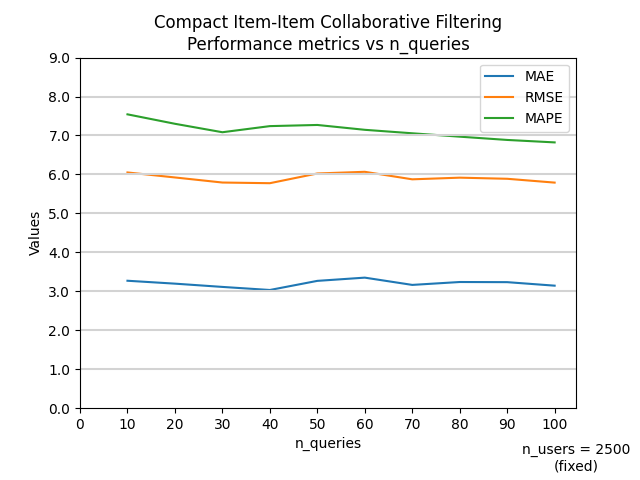
\includegraphics[width=9cm]{Data Mining/images/compact_item_item_queries.png}
\caption{Evaluation metrics of Compact Item-Item CF, varying number of queries}
\label{fig:Compact Item-Item CF, varying queries}
\end{figure}




\subsubsection{Compact User-User CF metrics values}
\label{sec:compact-user-user-metrics}

The experimental evaluation of Compact User-User Collaborative Filtering \textbf{confirmed what the theory says} about this topic, even in this specific setting: Item-Item CF often works better than User-User CF. As shown in Figures \ref{fig:Compact User-User CF, varying users} and \ref{fig:Compact User-User CF, varying queries}, all three metrics considered have significantly higher values than the values described in the previous section.

\begin{figure}[h!]
\centering
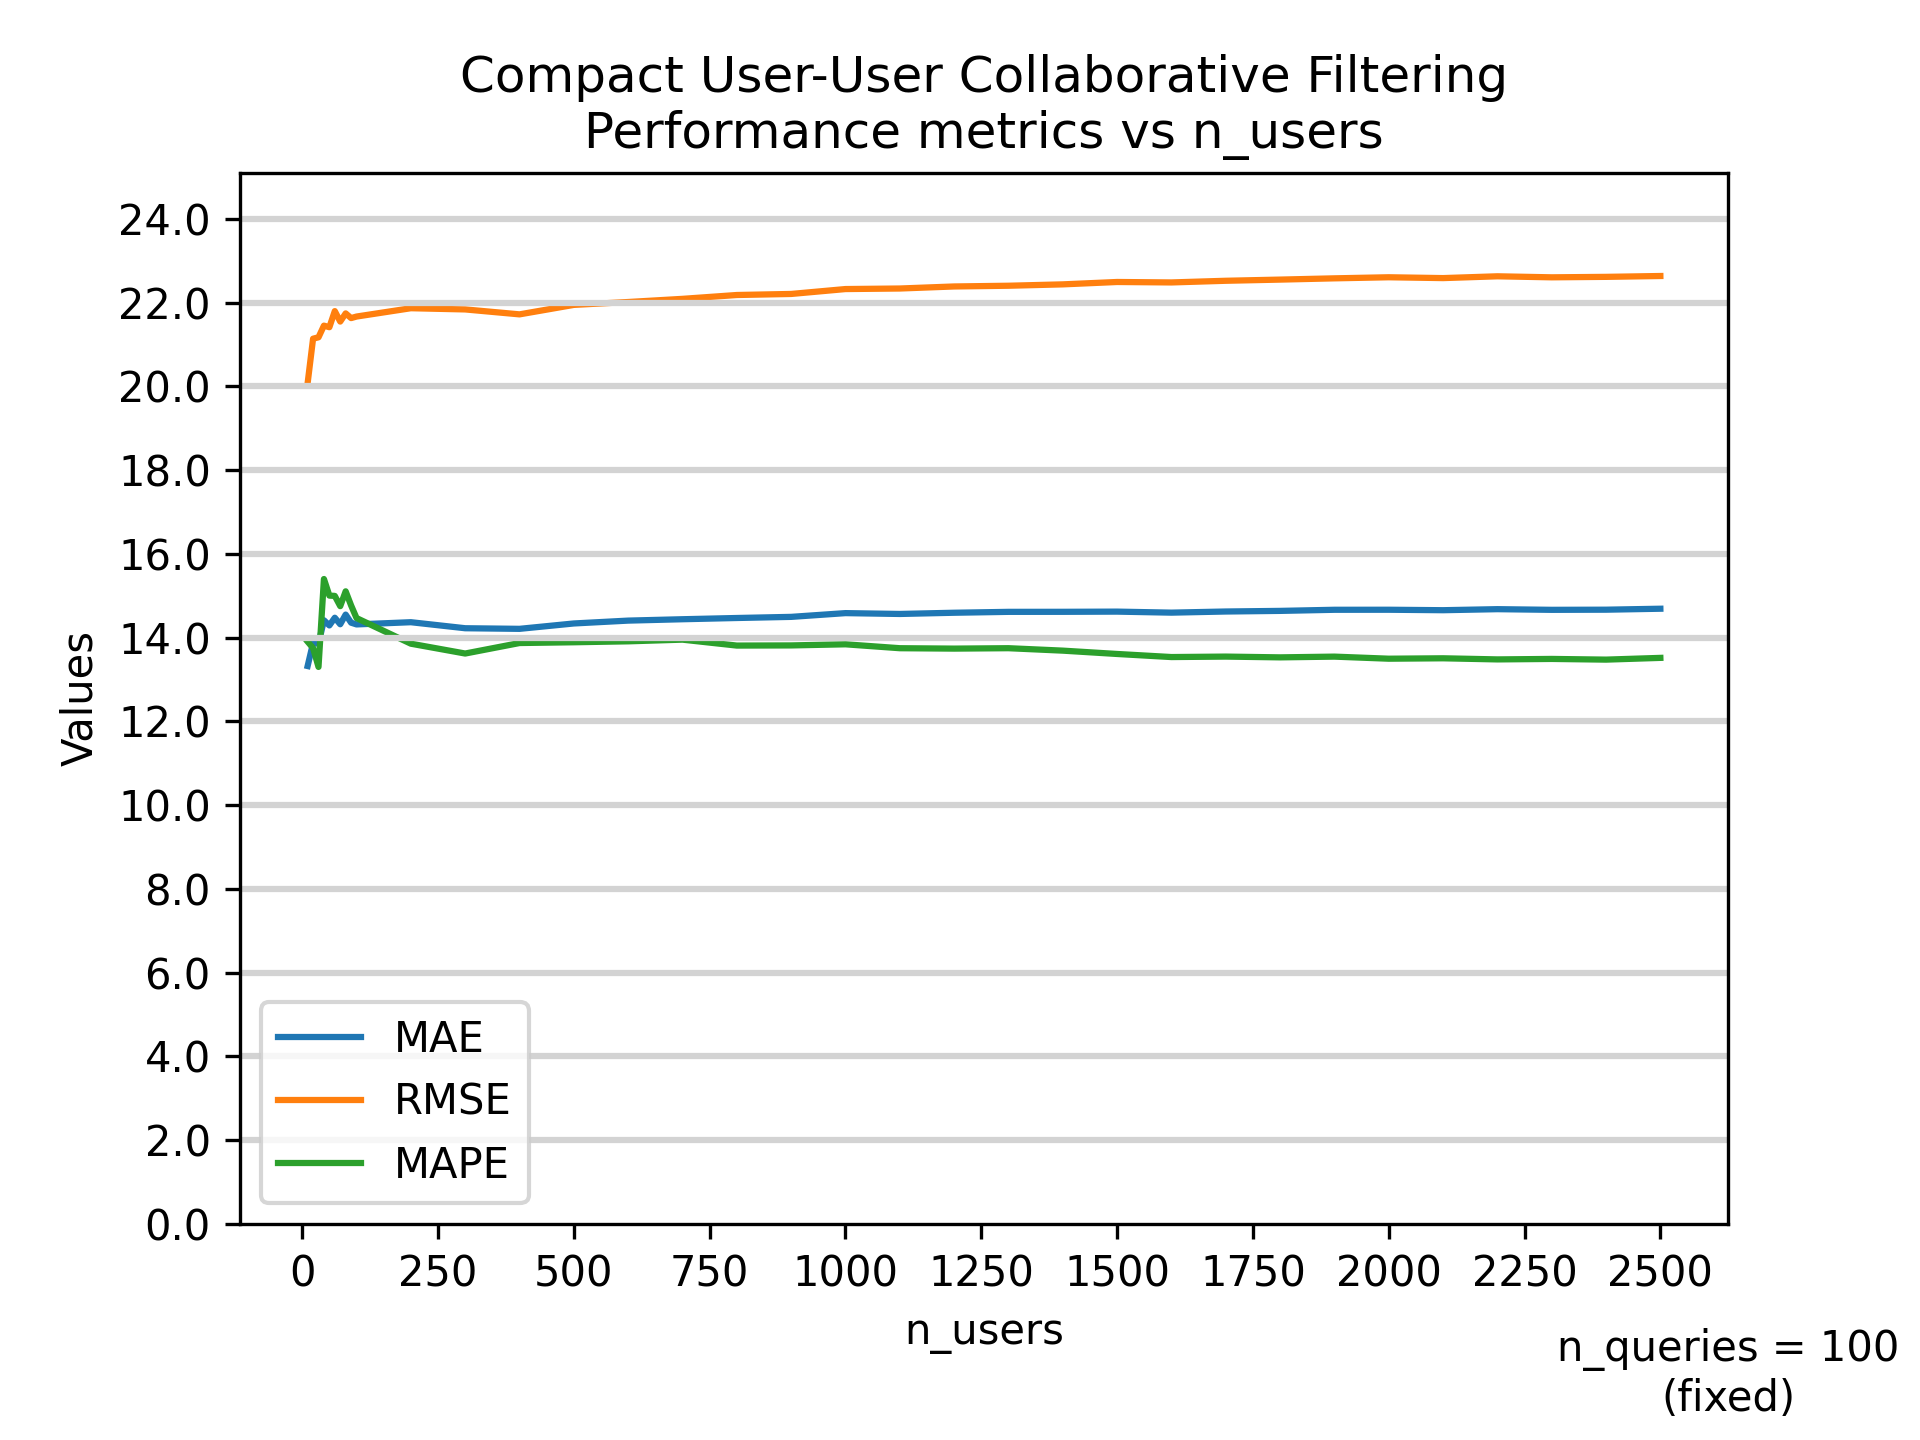
\includegraphics[width=9cm]{Data Mining/images/compact_user_user_users.png}
\caption{Evaluation metrics of Compact User-User CF, varying number of users}
\label{fig:Compact User-User CF, varying users}
\end{figure}

\begin{figure}[h!]
\centering
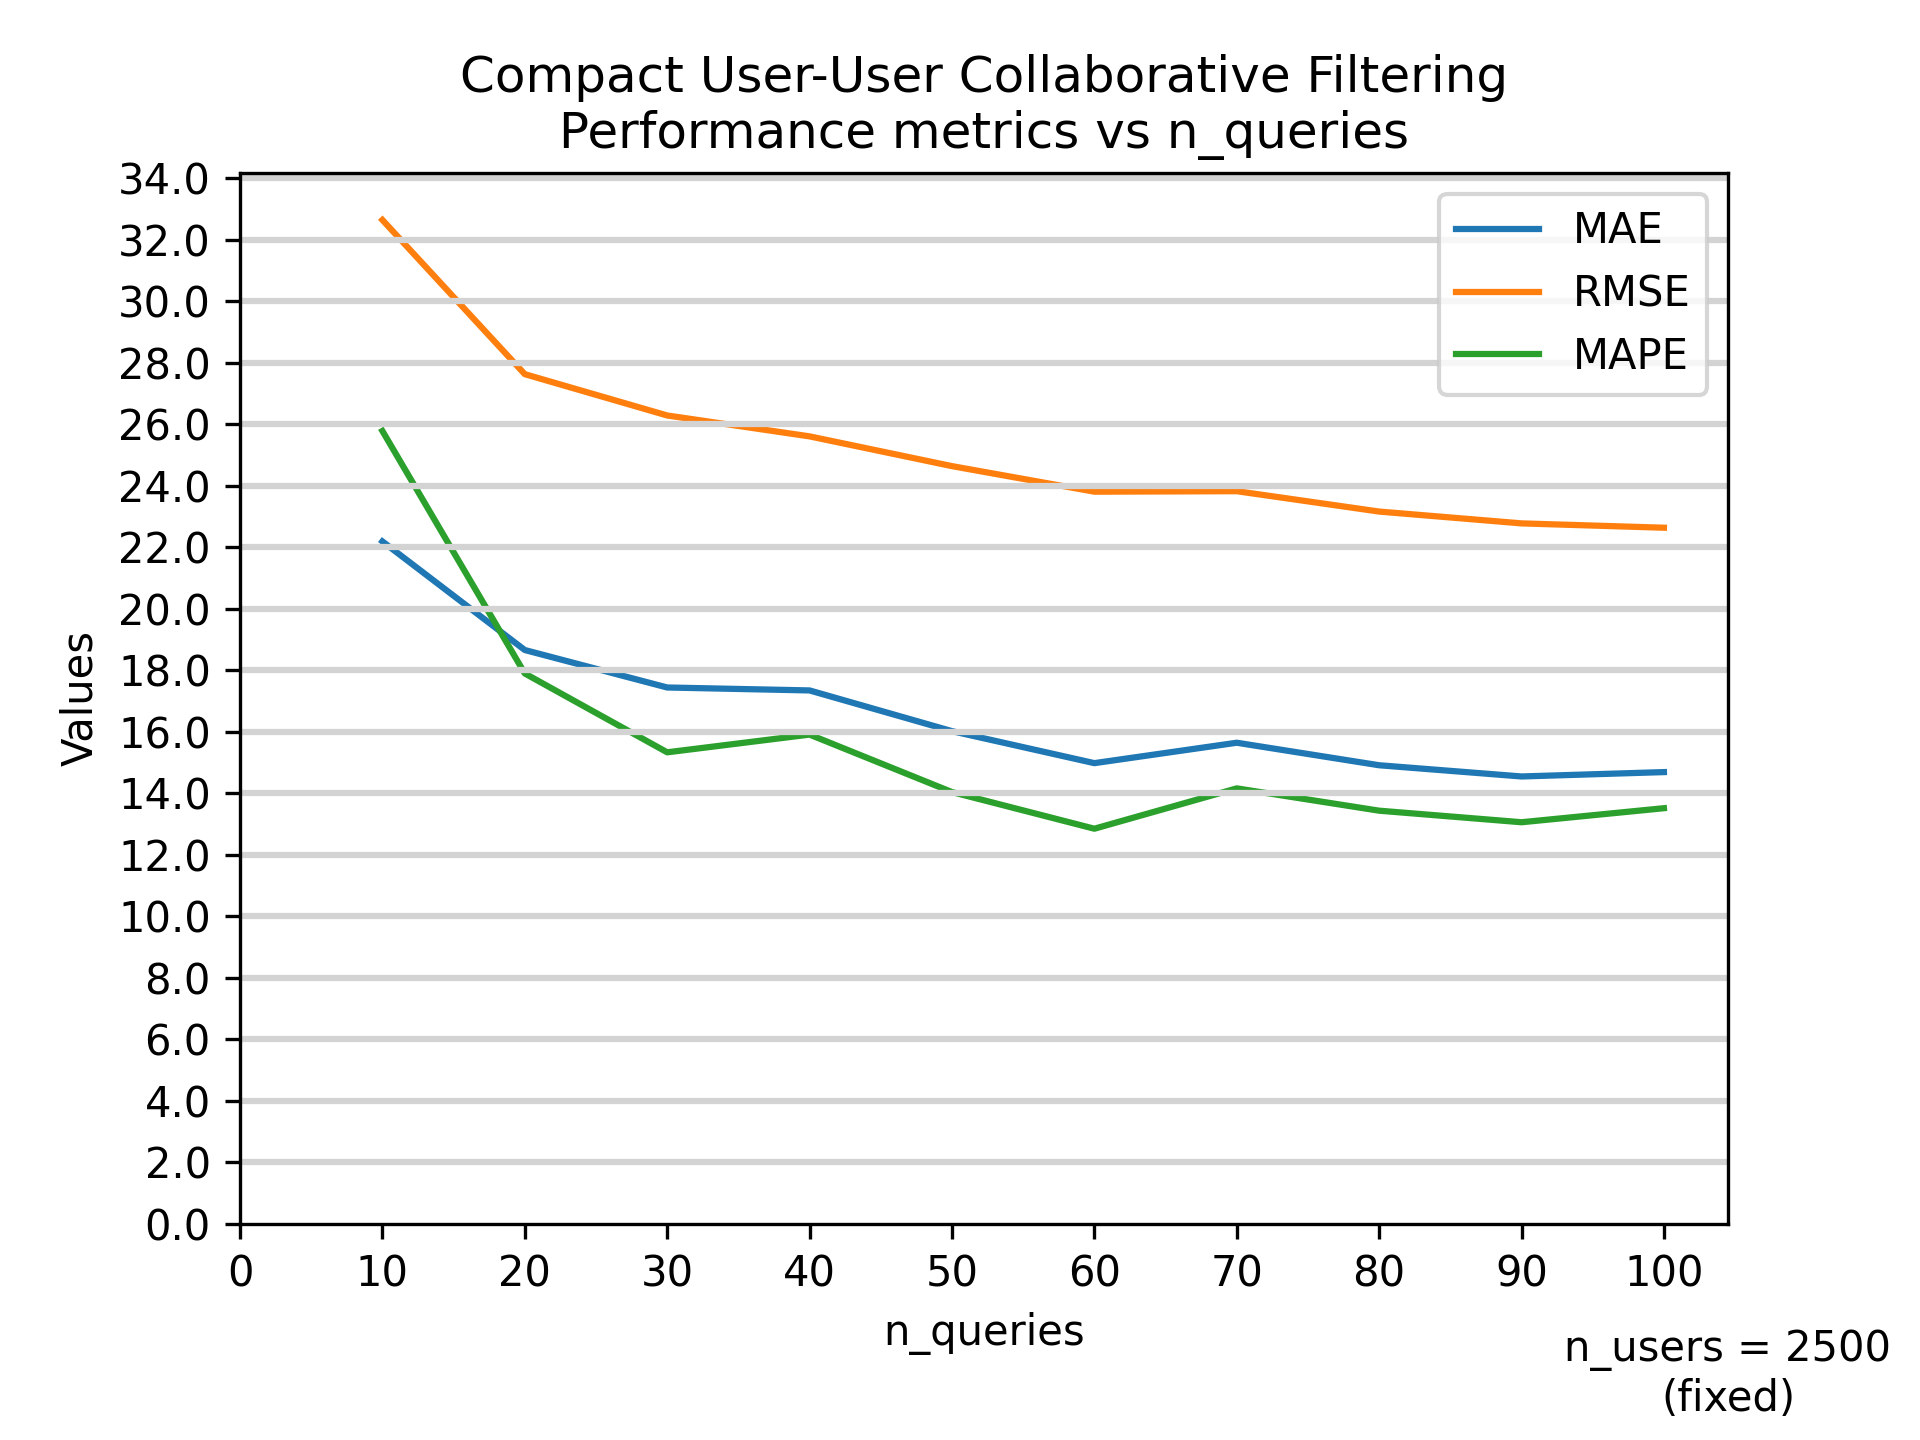
\includegraphics[width=9cm]{Data Mining/images/compact_user_user_queries.png}
\caption{Evaluation metrics of Compact User-User CF, varying number of queries}
\label{fig:Compact User-User CF, varying queries}
\end{figure}


\subsubsection{Expanded Item-Item CF metrics values}

When tested, this component behaves similarly to the previous ones, but the main difference is that it reaches a performance plateau for all three evaluation metrics at a much \textbf{faster} "speed", that is, after only 15 users considered, as shown in Table \ref{tab:expanded Item-Item CF, nitems fixed} and in Figure \ref{fig:Expanded Item-Item CF, varying users} (representing only data considering the first 100 users).


\begin{table}[h!]
    \centering
    \begin{tabular}{ |p{2cm}||p{1.5cm}|p{1.5cm}|p{1.5cm}|  }
         \hline
         \multicolumn{4}{|c|}{Expanded Item-Item CF, n\_items (7669) fixed } \\
         \hline
         \textbf{N\_USERS}& \textbf{MAE} &\textbf{RMSE} &\textbf{MAPE}\\
         \hline
         2 & 7.3249 & 16.2740  & 13.6591\\
         5 & 2.94 & 5.4743  & 5.9994\\
         15 & 2.616  & 4.8884  & 5.6474\\
         50 & 2.6342 & 4.9518 & 5.7490\\
         100 & 2.641  & 4.9109 & 5.7269\\
         200 & 2.6540 & 4.9446 & 5.7057\\
         1250 & 2.7587 & 5.1672 & 5.9894\\
         \textbf{2500} & \textbf{2.7630} & \textbf{5.1779} & \textbf{5.9939}\\
 
         \hline
    \end{tabular}
    \caption{Expanded Item-Item CF, n\_items fixed}
    \label{tab:expanded Item-Item CF, nitems fixed}
\end{table}


\begin{figure}[h!]
\centering
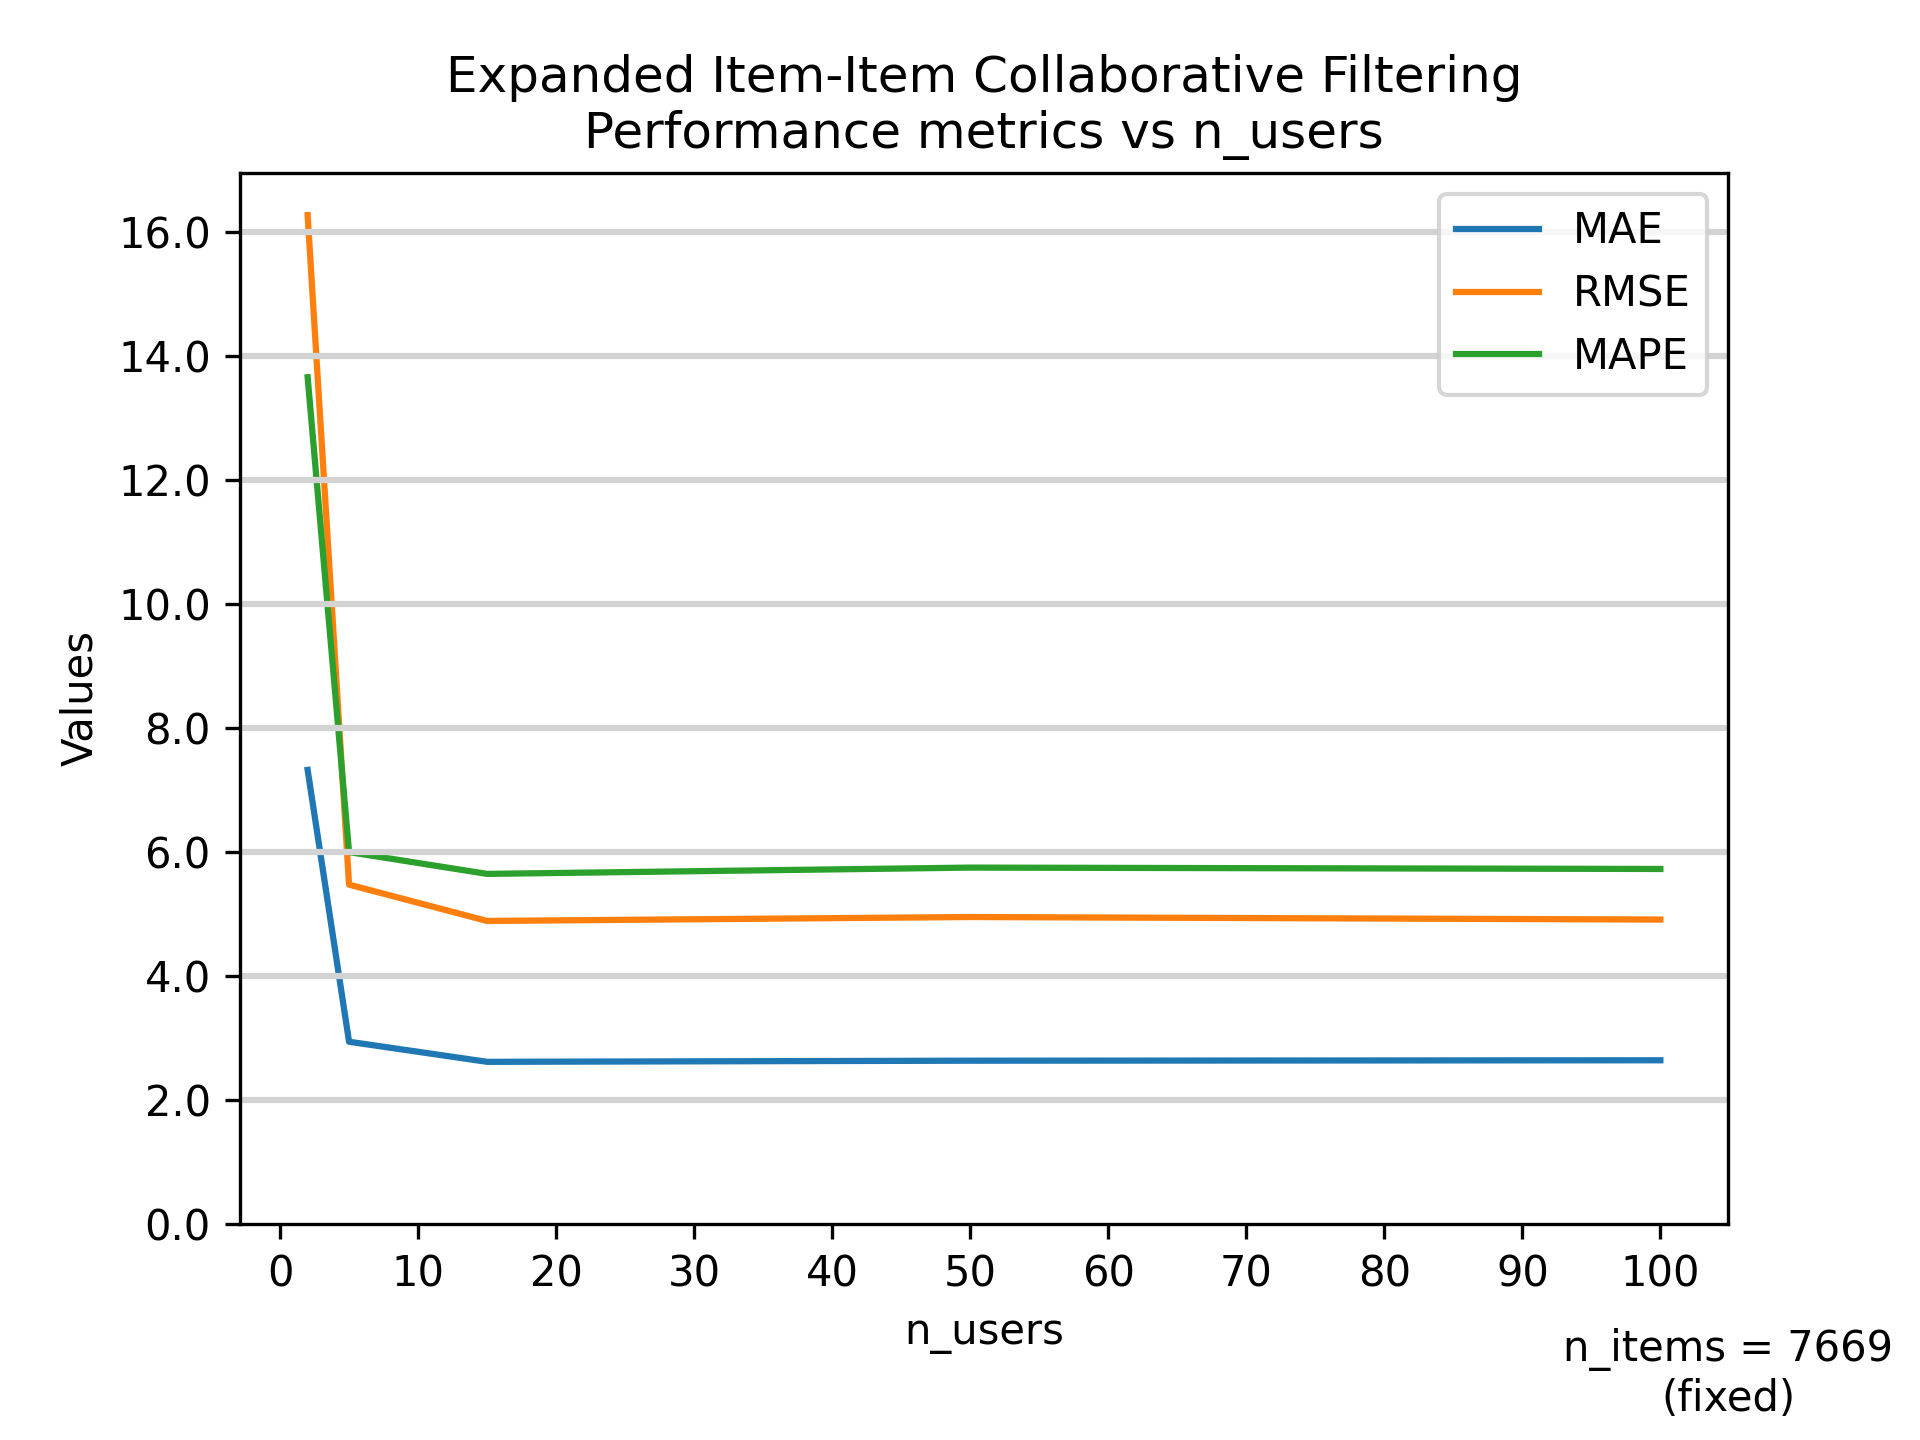
\includegraphics[width=9cm]{Data Mining/images/expanded_item_item_users.png}
\caption{Evaluation metrics of Expanded Item-Item CF, varying number of users}
\label{fig:Expanded Item-Item CF, varying users}
\end{figure}




\subsection{Baseline selection}
\subsubsection{Part A}
\label{sec:baseline-partA}
Among all the approaches that were implemented during the project development, it was chosen as baseline to be used as comparison meter for the PART\_A, the \textbf{Compact} (Standard) \textbf{Item-Item Collaborative Filtering} component described in the Section \ref{sec:compact-item-item-cf-solution}, mainly due to the implementation availability and popularity of that approach in Data Science related works.
\subsubsection{Part B}
Regarding the baseline chosen in order to allow a comparison with the solution described in the subchapter \ref{ch:5.7.2} for the PART\_B, it was decided to expand, as described in the Algorithm \ref{alg:partb_ch4.5.2}, the \textit{Complete Utility Matrix} obtained by running the \textbf{Expanded Item-Item Collaborative Filtering} on the Utility Matrix $U$. The obtained Complete \textit{user-RelationalItem\_utility\_matrix} was used to compute the ratings regarding the new queries.


\subsection{Experimental results accomplished by hybrid solution}
\subsubsection{Part A}
\label{sec:results-hybrid-parta}
To compare the baseline chosen in section \ref{sec:baseline-partA} to the final solution, two main strategies were put in place:  evaluate their ability in correctly \textbf{filling} the Utility Matrix $U$ and, to give the task a more practical meaning, the approaches were also compared in the efficiency in \textbf{finding} the \textit{TOP\_K} queries belonging to the users of the User Set $US$ considered.

Concerning the ability in filling the Utility Matrix $U$, it was actually computed, using both the solution and the baseline method, a \textit{Complete Utility Matrix}, which was then compared to the \textit{Real Complete} one, computed as described in the subsection \ref{ch:5.2}. Referring to the Table \ref{tab:part-a-baseline}, it is possible to see that with the current dataset under consideration (considering N\_QUERIES = 100, N\_USERS = 2500), the proposed solution \textbf{performs slightly better} than the baseline in \textbf{all} of the evaluation metrics proposed.

The configuration parameters for the hybrid solution are:
\begin{itemize}
    \item THRESHOLD\_1 = 200.0
    \item THRESHOLD\_2 = 1000.0
    \item WEIGHT\_1 = 0.75
    \item WEIGHT\_2 = 0.5
    \item WEIGHT\_3 = 0.25
\end{itemize}
    

\begin{table}[h!]
    \centering
    \begin{tabular}{ |p{2cm}||p{1.5cm}|p{1.5cm}|p{1.5cm}|  }
         \hline
         \multicolumn{4}{|c|}{PART A - Utility Matrix: Compact Item-Item CF vs. Hybrid} \\
         \hline
         \textbf{Method}& \textbf{MAE} &\textbf{RMSE} &\textbf{MAPE}\\
         \hline

         \textbf{Baseline} & 3.1420 & 5.7890 & 6.8218\\
         \textbf{Final solution} & \textbf{2.7446} & \textbf{5.1184} & \textbf{5.9671}\\
 
         \hline
    \end{tabular}
    \caption{PART A - Utility Matrix: Baseline vs. Final solution}
    \label{tab:part-a-baseline}
\end{table}


In terms of the second proposed comparison, the \textit{TOP\_K} queries from both the \textit{Complete Utility Matrix} computed by the final solution and the baseline are retrieved. After those query identifiers have been stored in \textbf{two sets} for each user (baseline, solution), they are compared with the actual \textit{TOP\_K} queries set belonging to the \textit{Real Complete Utility Matrix} from the dataset, using the \textbf{Jaccard similarity coefficient} as distance. It should be remarked that the higher the value, the more similar the two sets are.
This distance is calculated considering multiple values of $K$.
The minimum, maximum and mean value of the Jaccard index for each value of $K$ considered are reported in Table \ref{tab:jaccard}.

A \textbf{Dot-Box plot}, represented in Figure \ref{fig:jaccard-topk-parta}, is used to visualize the distribution of the gathered data, showing the median (middle line in the box), 25th quartile (lower edge of the box), 75th quartile (higher edge of the box), and the outliers. The dots, in addition, give a sense of how many data points lie within each group.  
As we can see in the figure, for the first 5 values of K, the lowest, median and highest values of the Jaccard index are the same for both the baseline and the solution. 
This suggests that there is basically \textbf{no advantage} in using a hybrid approach with respect to a standard one, for low K values, i.e., small sets of highest rated queries. 
Starting from the value K = 10, median, 25th quartile and 75th quartile values related to the solution are \textbf{higher}, as it can be seen by the middle line, lower and higher edge of the boxes.
It could be also noted that, for all the values of K considered, as Table \ref{tab:jaccard} shows, the mean of the Jaccard similarity coefficient is always \textbf{slightly higher} for the solution.


\begin{table}[]
\begin{tabular}{l|lll|}
\cline{2-4}
                                          & \multicolumn{3}{l|}{Jaccard similarity coefficient, versus real dataset}    \\ \hline
\multicolumn{1}{|l|}{\textbf{TOP\_K}}              & \multicolumn{1}{l|}{\textbf{Min}}       & \multicolumn{1}{l|}{\textbf{Max}}       & \textbf{Mean}      \\ \hline
\multicolumn{1}{|l|}{\multirow{2}{*}{1}}  & \multicolumn{1}{l|}{C: 0.0}    & \multicolumn{1}{l|}{C: 1.0}    & C: 0.3176 \\ \cline{2-4} 
\multicolumn{1}{|l|}{}                    & \multicolumn{1}{l|}{H: 0.0}    & \multicolumn{1}{l|}{H: 1.0}    & H: 0.3296 \\ \hline
\multicolumn{1}{|l|}{\multirow{2}{*}{2}}  & \multicolumn{1}{l|}{C: 0.0}    & \multicolumn{1}{l|}{C: 1.0}    & C: 0.2621 \\ \cline{2-4} 
\multicolumn{1}{|l|}{}                    & \multicolumn{1}{l|}{H: 0.0}    & \multicolumn{1}{l|}{H: 1.0}    & H: 0.2814 \\ \hline
\multicolumn{1}{|l|}{\multirow{2}{*}{3}}  & \multicolumn{1}{l|}{C: 0.0}    & \multicolumn{1}{l|}{C: 1.0}    & C: 0.2504 \\ \cline{2-4} 
\multicolumn{1}{|l|}{}                    & \multicolumn{1}{l|}{H: 0.0}    & \multicolumn{1}{l|}{H: 1.0}    & H: 0.2753 \\ \hline
\multicolumn{1}{|l|}{\multirow{2}{*}{4}}  & \multicolumn{1}{l|}{C: 0.0}    & \multicolumn{1}{l|}{C: 1.0}    & C: 0.2529 \\ \cline{2-4} 
\multicolumn{1}{|l|}{}                    & \multicolumn{1}{l|}{H: 0.0}    & \multicolumn{1}{l|}{H: 1.0}    & H: 0.2786 \\ \hline
\multicolumn{1}{|l|}{\multirow{2}{*}{5}}  & \multicolumn{1}{l|}{C: 0.0}    & \multicolumn{1}{l|}{C: 1.0}    & C: 0.2606 \\ \cline{2-4} 
\multicolumn{1}{|l|}{}                    & \multicolumn{1}{l|}{H: 0.0}    & \multicolumn{1}{l|}{H: 1.0}    & H: 0.2862 \\ \hline
\multicolumn{1}{|l|}{\multirow{2}{*}{10}} & \multicolumn{1}{l|}{C: 0.0}    & \multicolumn{1}{l|}{C: 0.8181} & C: 0.2821 \\ \cline{2-4} 
\multicolumn{1}{|l|}{}                    & \multicolumn{1}{l|}{H: 0.0}    & \multicolumn{1}{l|}{H: 0.8181} & H: 0.3115 \\ \hline
\multicolumn{1}{|l|}{\multirow{2}{*}{15}} & \multicolumn{1}{l|}{C: 0.0}    & \multicolumn{1}{l|}{C: 0.7647} & C: 0.3098 \\ \cline{2-4} 
\multicolumn{1}{|l|}{}                    & \multicolumn{1}{l|}{H: 0.0}    & \multicolumn{1}{l|}{H: 0.875}  & H: 0.3373 \\ \hline
\multicolumn{1}{|l|}{\multirow{2}{*}{20}} & \multicolumn{1}{l|}{C: 0.0256} & \multicolumn{1}{l|}{C: 0.7391} & C: 0.3436 \\ \cline{2-4} 
\multicolumn{1}{|l|}{}                    & \multicolumn{1}{l|}{H: 0.0526} & \multicolumn{1}{l|}{H: 0.8181} & H: 0.3696 \\ \hline
\multicolumn{1}{|l|}{\multirow{2}{*}{30}} & \multicolumn{1}{l|}{C: 0.1538} & \multicolumn{1}{l|}{C: 0.8181} & C: 0.4309 \\ \cline{2-4} 
\multicolumn{1}{|l|}{}                    & \multicolumn{1}{l|}{H: 0.1320} & \multicolumn{1}{l|}{H: 0.7647} & H: 0.4576 \\ \hline
\end{tabular}
\caption{PART A - TOP-K queries: Baseline (C) vs. Final Solution (H)}
\label{tab:jaccard}
\end{table}



\begin{figure}[h!]
\centering
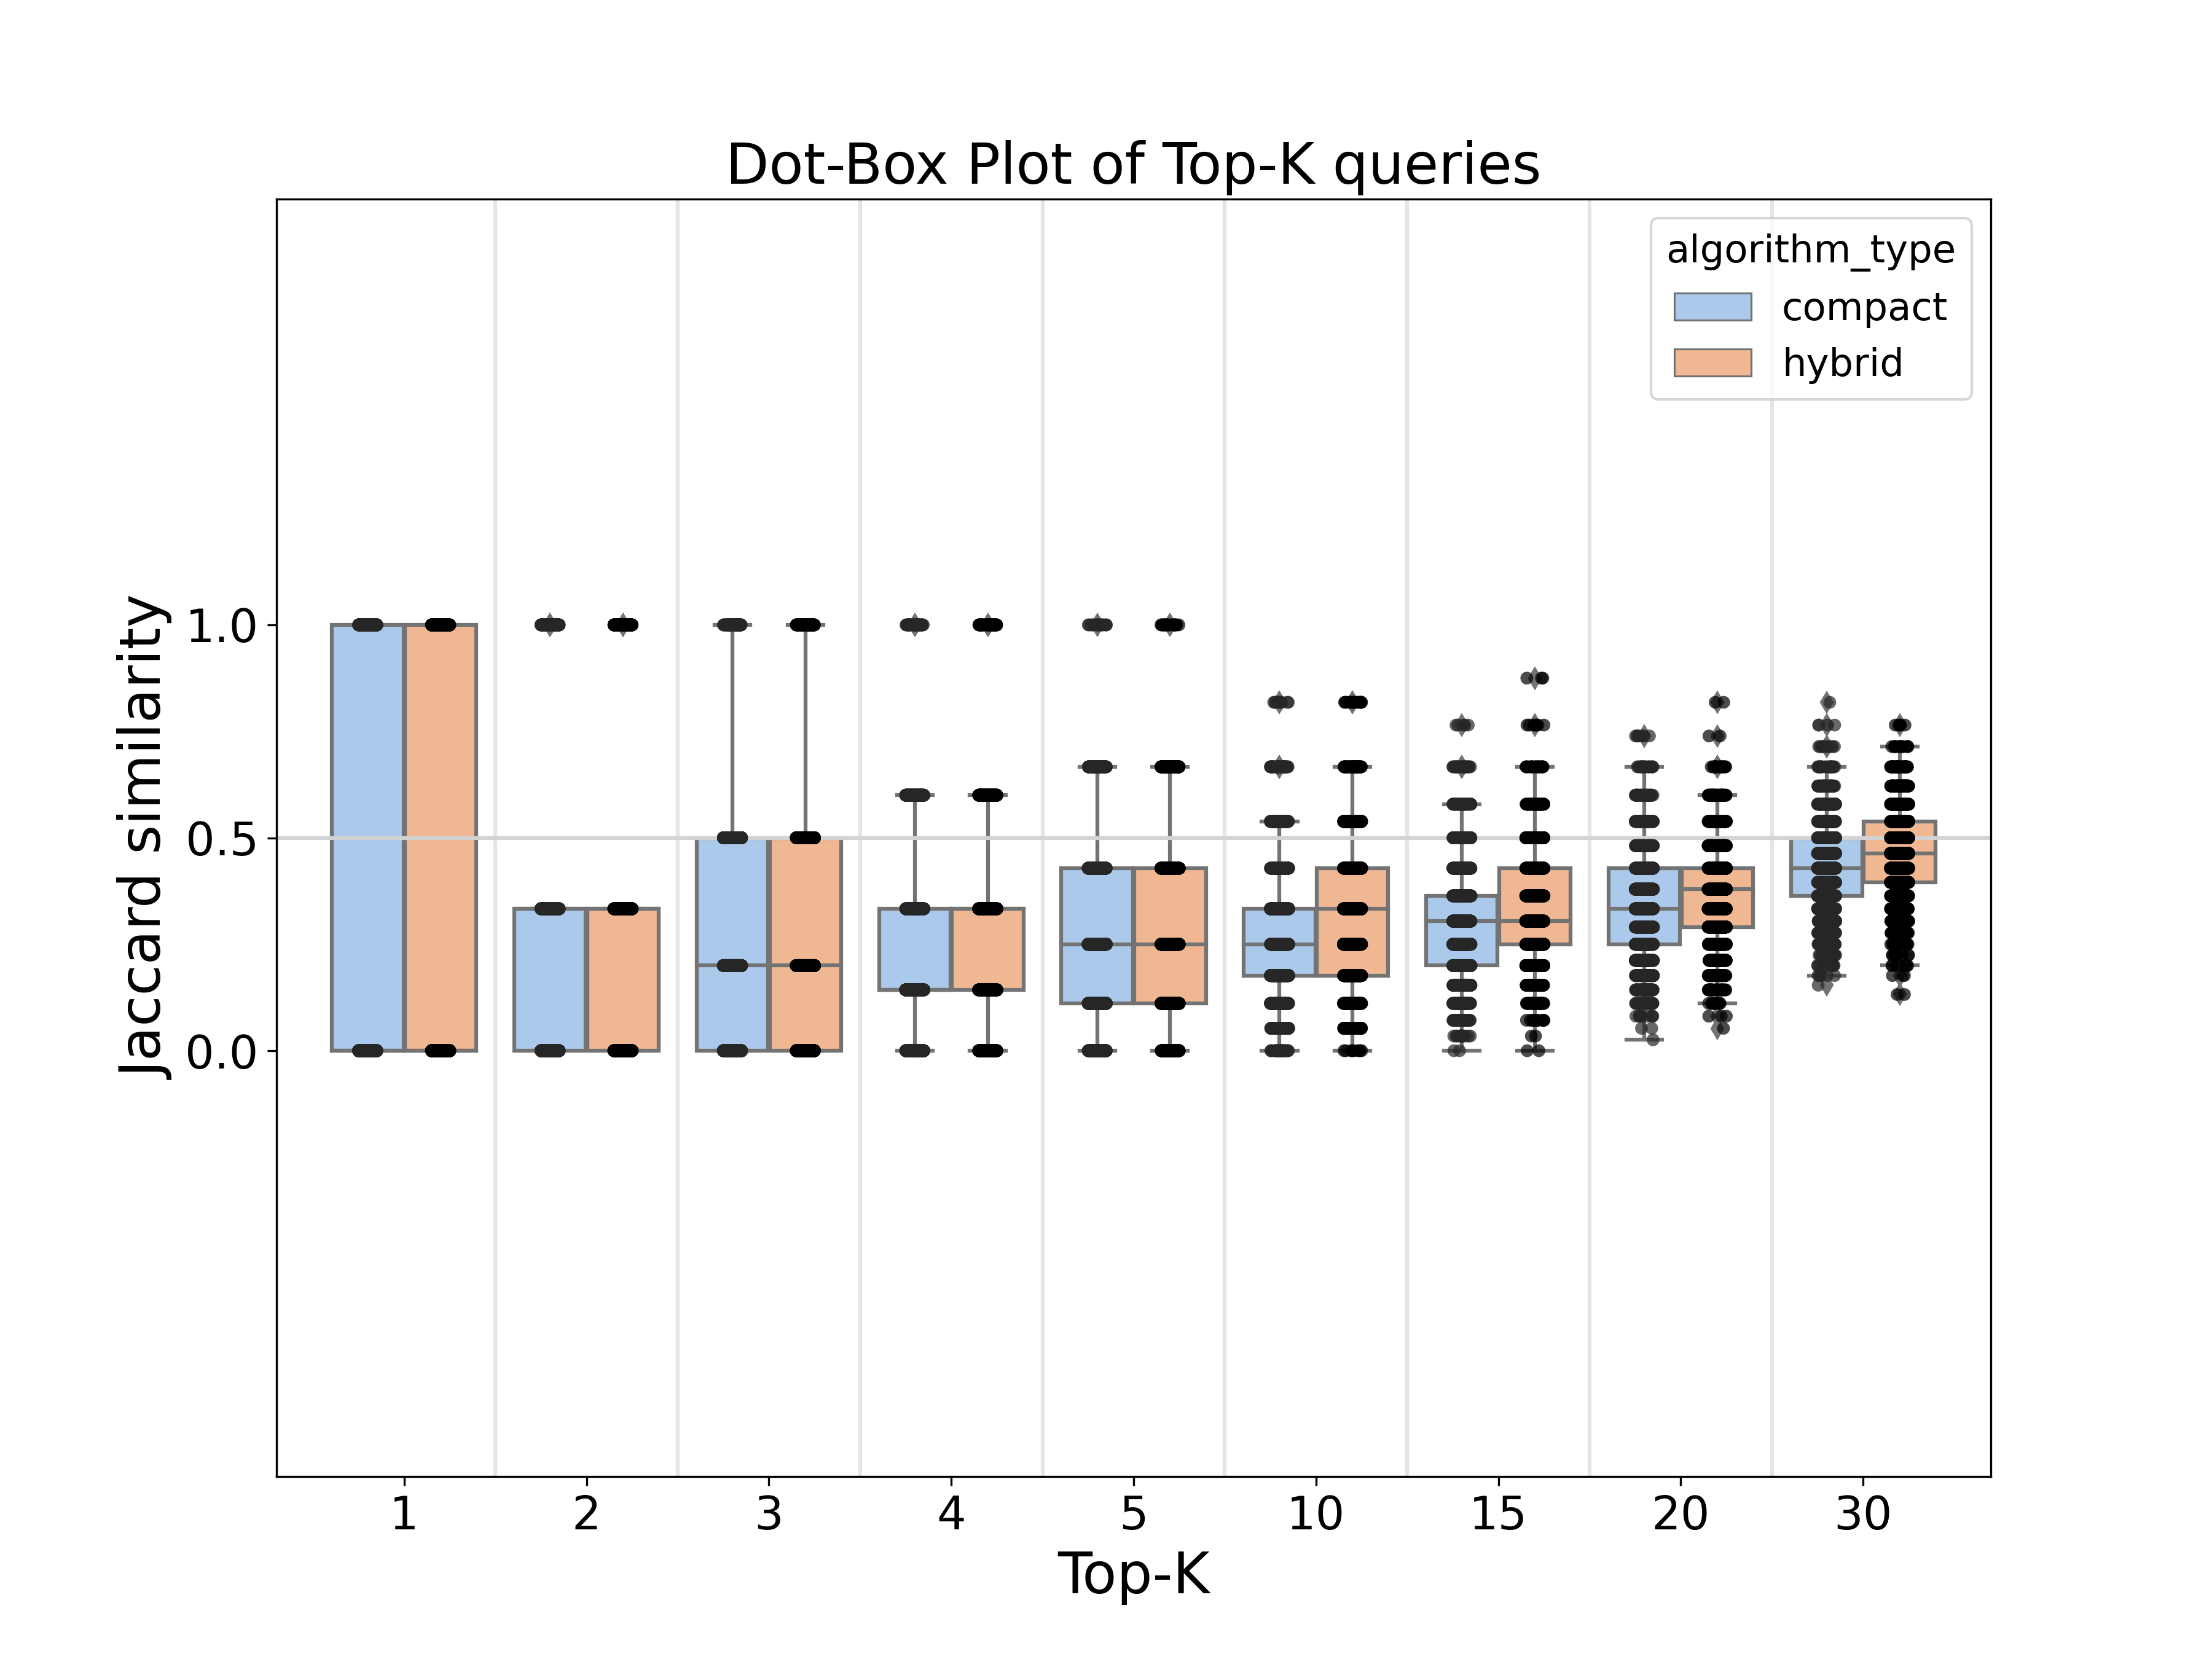
\includegraphics[width=9cm]{Data Mining/images/jaccard_part_a.png}
\caption{PART A - Jaccard similarity for the Top-K queries sets}
\label{fig:jaccard-topk-parta}
\end{figure}




\subsubsection{Part B} \label{ch:5.7.2}
Regarding the comparison of the second baseline chosen with our solution, a similar approach to the one described in the subsection \ref{sec:results-hybrid-parta} was followed. So, given some new and unseen queries, there were built 3 new utility matrices:
\begin{itemize}
    \item A \textit{New Real Complete Utility Matrix}, obtained by comparing the results of each new query with the existing users profiles as described in the Algorithm \ref{alg:users-queries score computation}.
    \item A \textit{Baseline Complete Utility Matrix}, obtained by computing a prediction for every user-query combination as described in the Algorithm \ref{alg:partb-ch4.5.1}. The intermediate \textit{Baseline User-Relational Item Utility Matrix} was the same obtained by the expansion described in the subchapter \ref{sub:expansion}  and the users and queries taken into account during the compression were the same of the \textit{New Real Complete Utility Matrix}.
    \item Another \textit{Hybrid Complete Utility Matrix} built by expanding and then compressing the Utility Matrix computed by our solution described in the subchapter \ref{sec:results-hybrid-parta}. The expansion was done considering the definition of the original Utility Matrix $U$ being part of our problem statement while the compression was done considering the new queries proposed during the PART\_B, as described in the subchapter \ref{ch:4.2.3}.
\end{itemize}

Once obtained those three Utility Matrices, the \textit{New Real Complete Utility Matrix} is compared with the baseline one and with the hybrid one (representing our solution), using the three evaluation metrics described in the subsection \ref{sec:evaluation-metrics}. The results are shown in Table \ref{tab:part-b-baseline} where it can be seen that the final solution has performed \textbf{slightly better} in 2 out of 3 evaluation metrics. However, the values gathered at this stage are all very similar to one another.



As done for the PART\_A, in order to evaluate the solution in a more practical term, the \textit{TOP\_K} queries from both the Complete Utility Matrix computed by the final solution and from baseline are retrieved. After those query identifiers have been stored in two sets for each user (baseline, solution), they are compared with the actual \textit{TOP\_K} queries set belonging to the Real Complete Utility Matrix that has been created for PART\_B, using the Jaccard similarity coefficient as distance.

As for PART\_A, the minimum, maximum and mean value of the Jaccard index for each value of K considered are reported in Table \ref{tab:jaccardB}.
Another \textbf{Dot-Box plot}, represented in Figure \ref{fig:jaccard-topk-partb}, is used to visualize the distribution of the data.
Looking at the latter, the results obtained are \textbf{nearly identical} for each value of k considered. One thing to note is that in the case of maximum k tested (25) the 25th quartile associated with the hybrid method has a slightly higher jaccard index than the 25th quartile associated with the expanded method.


\begin{table}[h!]
    \centering
    \begin{tabular}{ |p{2cm}||p{1.5cm}|p{1.5cm}|p{1.5cm}|  }
         \hline
         \multicolumn{4}{|c|}{PART B - Utility Matrix: Expanded Item-Item CF vs. Hybrid} \\
         \hline
         \textbf{Method}& \textbf{MAE} &\textbf{RMSE} &\textbf{MAPE}\\
         \hline

         \textbf{Baseline} & 4.0507  & 6.1362  &  \textbf{8.6332}\\
         \textbf{Final solution} & \textbf{4.040864} & \textbf{6.1086} & 8.6342 \\
 
         \hline
    \end{tabular}
    \caption{PART B - Utility Matrix: Baseline vs. Final solution}
    \label{tab:part-b-baseline}
\end{table}


\begin{table}[]
\begin{tabular}{l|lll|}
\cline{2-4}
                                          & \multicolumn{3}{l|}{Jaccard similarity coefficient, versus real dataset}    \\ \hline
\multicolumn{1}{|l|}{\textbf{TOP\_K}}              & \multicolumn{1}{l|}{\textbf{Min}}       & \multicolumn{1}{l|}{\textbf{Max}}       & \textbf{Mean}      \\ \hline
\multicolumn{1}{|l|}{\multirow{2}{*}{1}}  & \multicolumn{1}{l|}{E: 0.0}    & \multicolumn{1}{l|}{E: 1.0}    & E: 0.1112 \\ \cline{2-4} 
\multicolumn{1}{|l|}{}                    & \multicolumn{1}{l|}{H: 0.0}    & \multicolumn{1}{l|}{H: 1.0}    & H: 0.1148 \\ \hline
\multicolumn{1}{|l|}{\multirow{2}{*}{2}}  & \multicolumn{1}{l|}{E: 0.0}    & \multicolumn{1}{l|}{E: 1.0}    & E: 0.1497 \\ \cline{2-4} 
\multicolumn{1}{|l|}{}                    & \multicolumn{1}{l|}{H: 0.0}    & \multicolumn{1}{l|}{H: 1.0}    & H: 0.1544 \\ \hline
\multicolumn{1}{|l|}{\multirow{2}{*}{3}}  & \multicolumn{1}{l|}{E: 0.0}    & \multicolumn{1}{l|}{E: 1.0}    & E: 0.1725 \\ \cline{2-4} 
\multicolumn{1}{|l|}{}                    & \multicolumn{1}{l|}{H: 0.0}    & \multicolumn{1}{l|}{H: 1.0}    & H: 0.1781 \\ \hline
\multicolumn{1}{|l|}{\multirow{2}{*}{4}}  & \multicolumn{1}{l|}{E: 0.0}    & \multicolumn{1}{l|}{E: 1.0}    & E: 0.1935 \\ \cline{2-4} 
\multicolumn{1}{|l|}{}                    & \multicolumn{1}{l|}{H: 0.0}    & \multicolumn{1}{l|}{H: 1.0}    & H: 0.1998 \\ \hline
\multicolumn{1}{|l|}{\multirow{2}{*}{5}}  & \multicolumn{1}{l|}{E: 0.0}    & \multicolumn{1}{l|}{E: 1.0}    & E: 0.2083 \\ \cline{2-4} 
\multicolumn{1}{|l|}{}                    & \multicolumn{1}{l|}{H: 0.0}    & \multicolumn{1}{l|}{H: 1.0}    & H: 0.2120 \\ \hline
\multicolumn{1}{|l|}{\multirow{2}{*}{10}} & \multicolumn{1}{l|}{E: 0.0}    & \multicolumn{1}{l|}{E: 0.8181} & E: 0.2722 \\ \cline{2-4} 
\multicolumn{1}{|l|}{}                    & \multicolumn{1}{l|}{H: 0.0}    & \multicolumn{1}{l|}{H: 0.8181} & H: 0.2802 \\ \hline
\multicolumn{1}{|l|}{\multirow{2}{*}{15}} & \multicolumn{1}{l|}{E: 0.0714}    & \multicolumn{1}{l|}{E: 0.7647} & E: 0.3596 \\ \cline{2-4} 
\multicolumn{1}{|l|}{}                    & \multicolumn{1}{l|}{H: 0.0714}    & \multicolumn{1}{l|}{H: 0.7647}  & H: 0.3671 \\ \hline
\multicolumn{1}{|l|}{\multirow{2}{*}{20}} & \multicolumn{1}{l|}{E: 0.3513} & \multicolumn{1}{l|}{E: 0.9230} & E: 0.5917 \\ \cline{2-4} 
\multicolumn{1}{|l|}{}                    & \multicolumn{1}{l|}{H: 0.3513} & \multicolumn{1}{l|}{H: 0.8518} & H: 0.5972 \\ \hline
\end{tabular}
\caption{PART B - TOP-K queries: Baseline (E) vs. Final Solution (H)}
\label{tab:jaccardB}
\end{table}

\begin{figure}[h!]
\centering
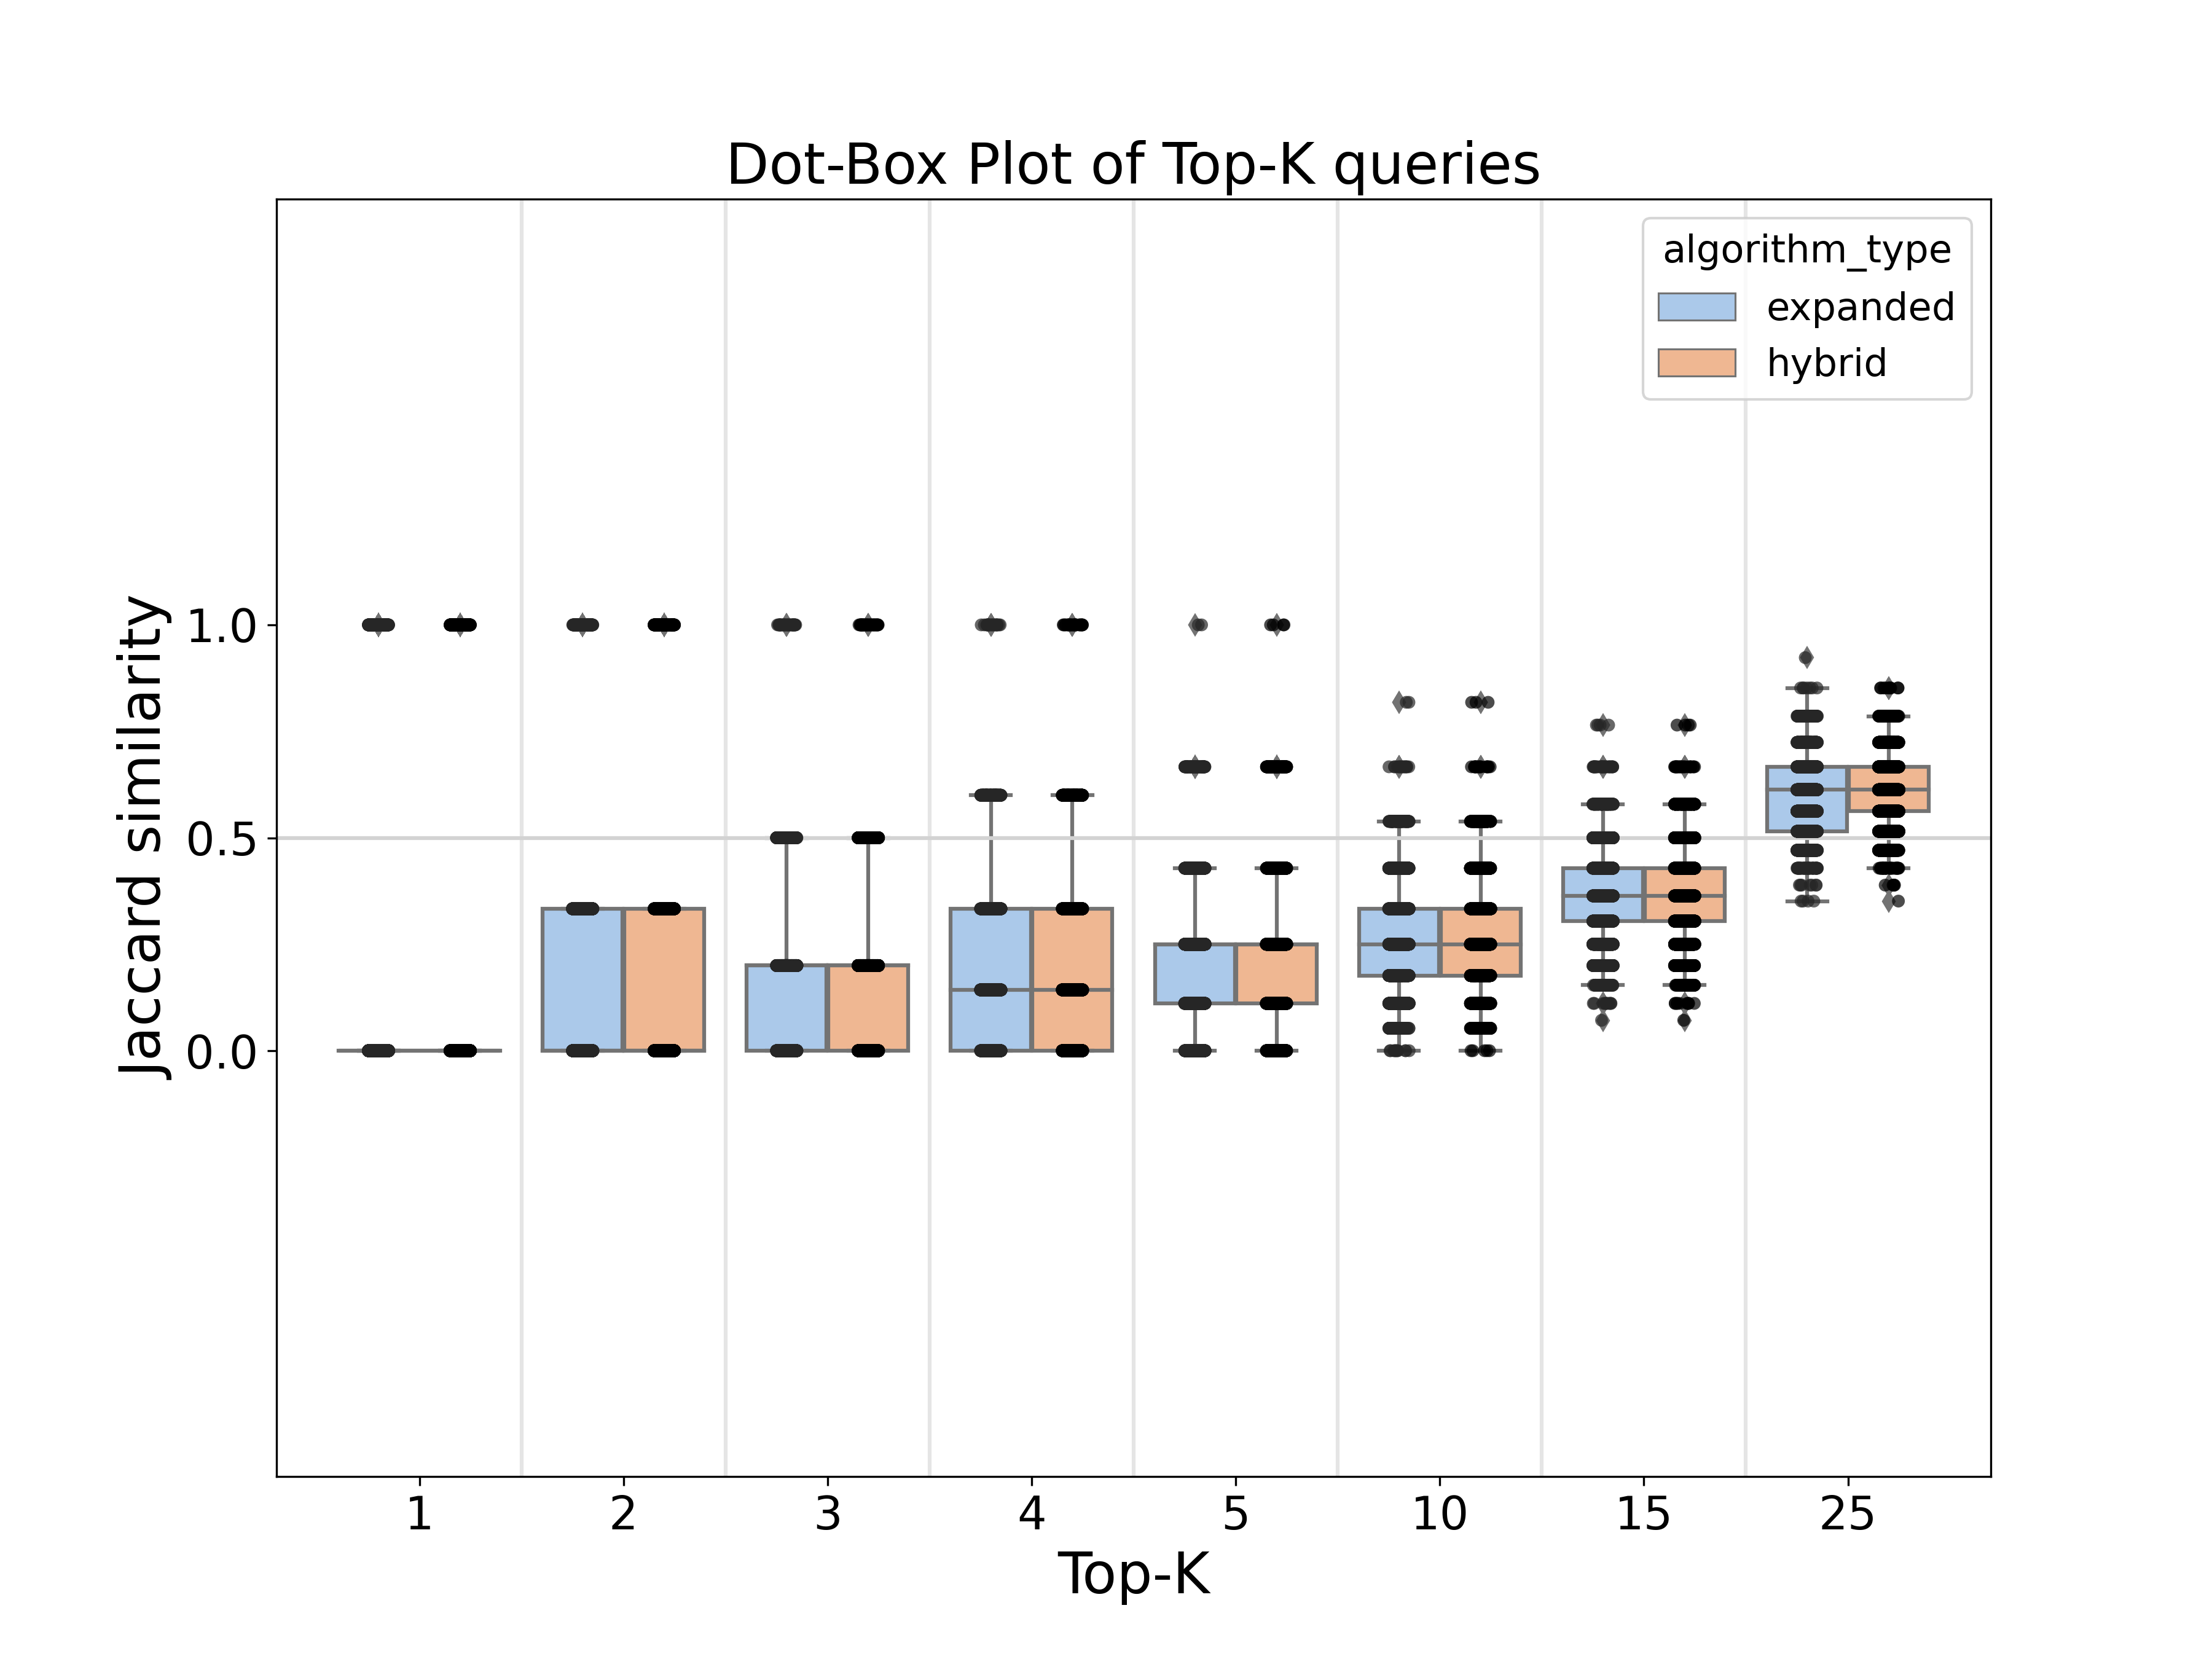
\includegraphics[width=9cm]{Data Mining/images/jaccard_part_b.png}
\caption{PART B - Jaccard similarity for the Top-K queries sets}
\label{fig:jaccard-topk-partb}
\end{figure}



